\chapter{Sputtering of Nanowires}

This chapter will investigate the sputtering of nanowires. The experiments were conducted together with Stefan Noack and are partially published in his master thesis \cite{noack_sputter_2014} and in Nano Letters \cite{johannes_anomalous_2015}.

% \section{First results in $Mn$ irradiated $GaAs$}

% Introduction by Mn in GaAs (JPhysD)


\section{Simulation results}
\label{sec:simsputering}

A good understanding of the sputtering of nanowires can be gained by looking at MC simulations results performed with \emph{iradina}. From the discussion of the Sigmund sputter model in chapter \ref{sec:ionsolid} a maximum is expected for a certain ion, ion energy and nanowire diameter combination. This is confirmed by MC simulations shown in figure \ref{sputtering_de}a and \ref{sputtering_de}b for the examples of $Xe^+$ and $Ar^+$ ions, respectively, homogeneously irradiating a $Si$ nanowire at an angle of $45^\circ$. Note that the color profile is not identical for both ions, as sputtering is about a factor of $2.5$ times larger for the denser collision cascades caused by the heavier $Xe^+$ ions. The white line indicates the ion range of the respective ion in bulk calculated with SRIM and projected on to $45^\circ$. The heavy $Xe^+$ has a much lower range than $Ar^+$ at the same energy. For both ions the maximum of the sputtering correlates very well with this ion range. 

\begin{figure}[th]
	\centering
		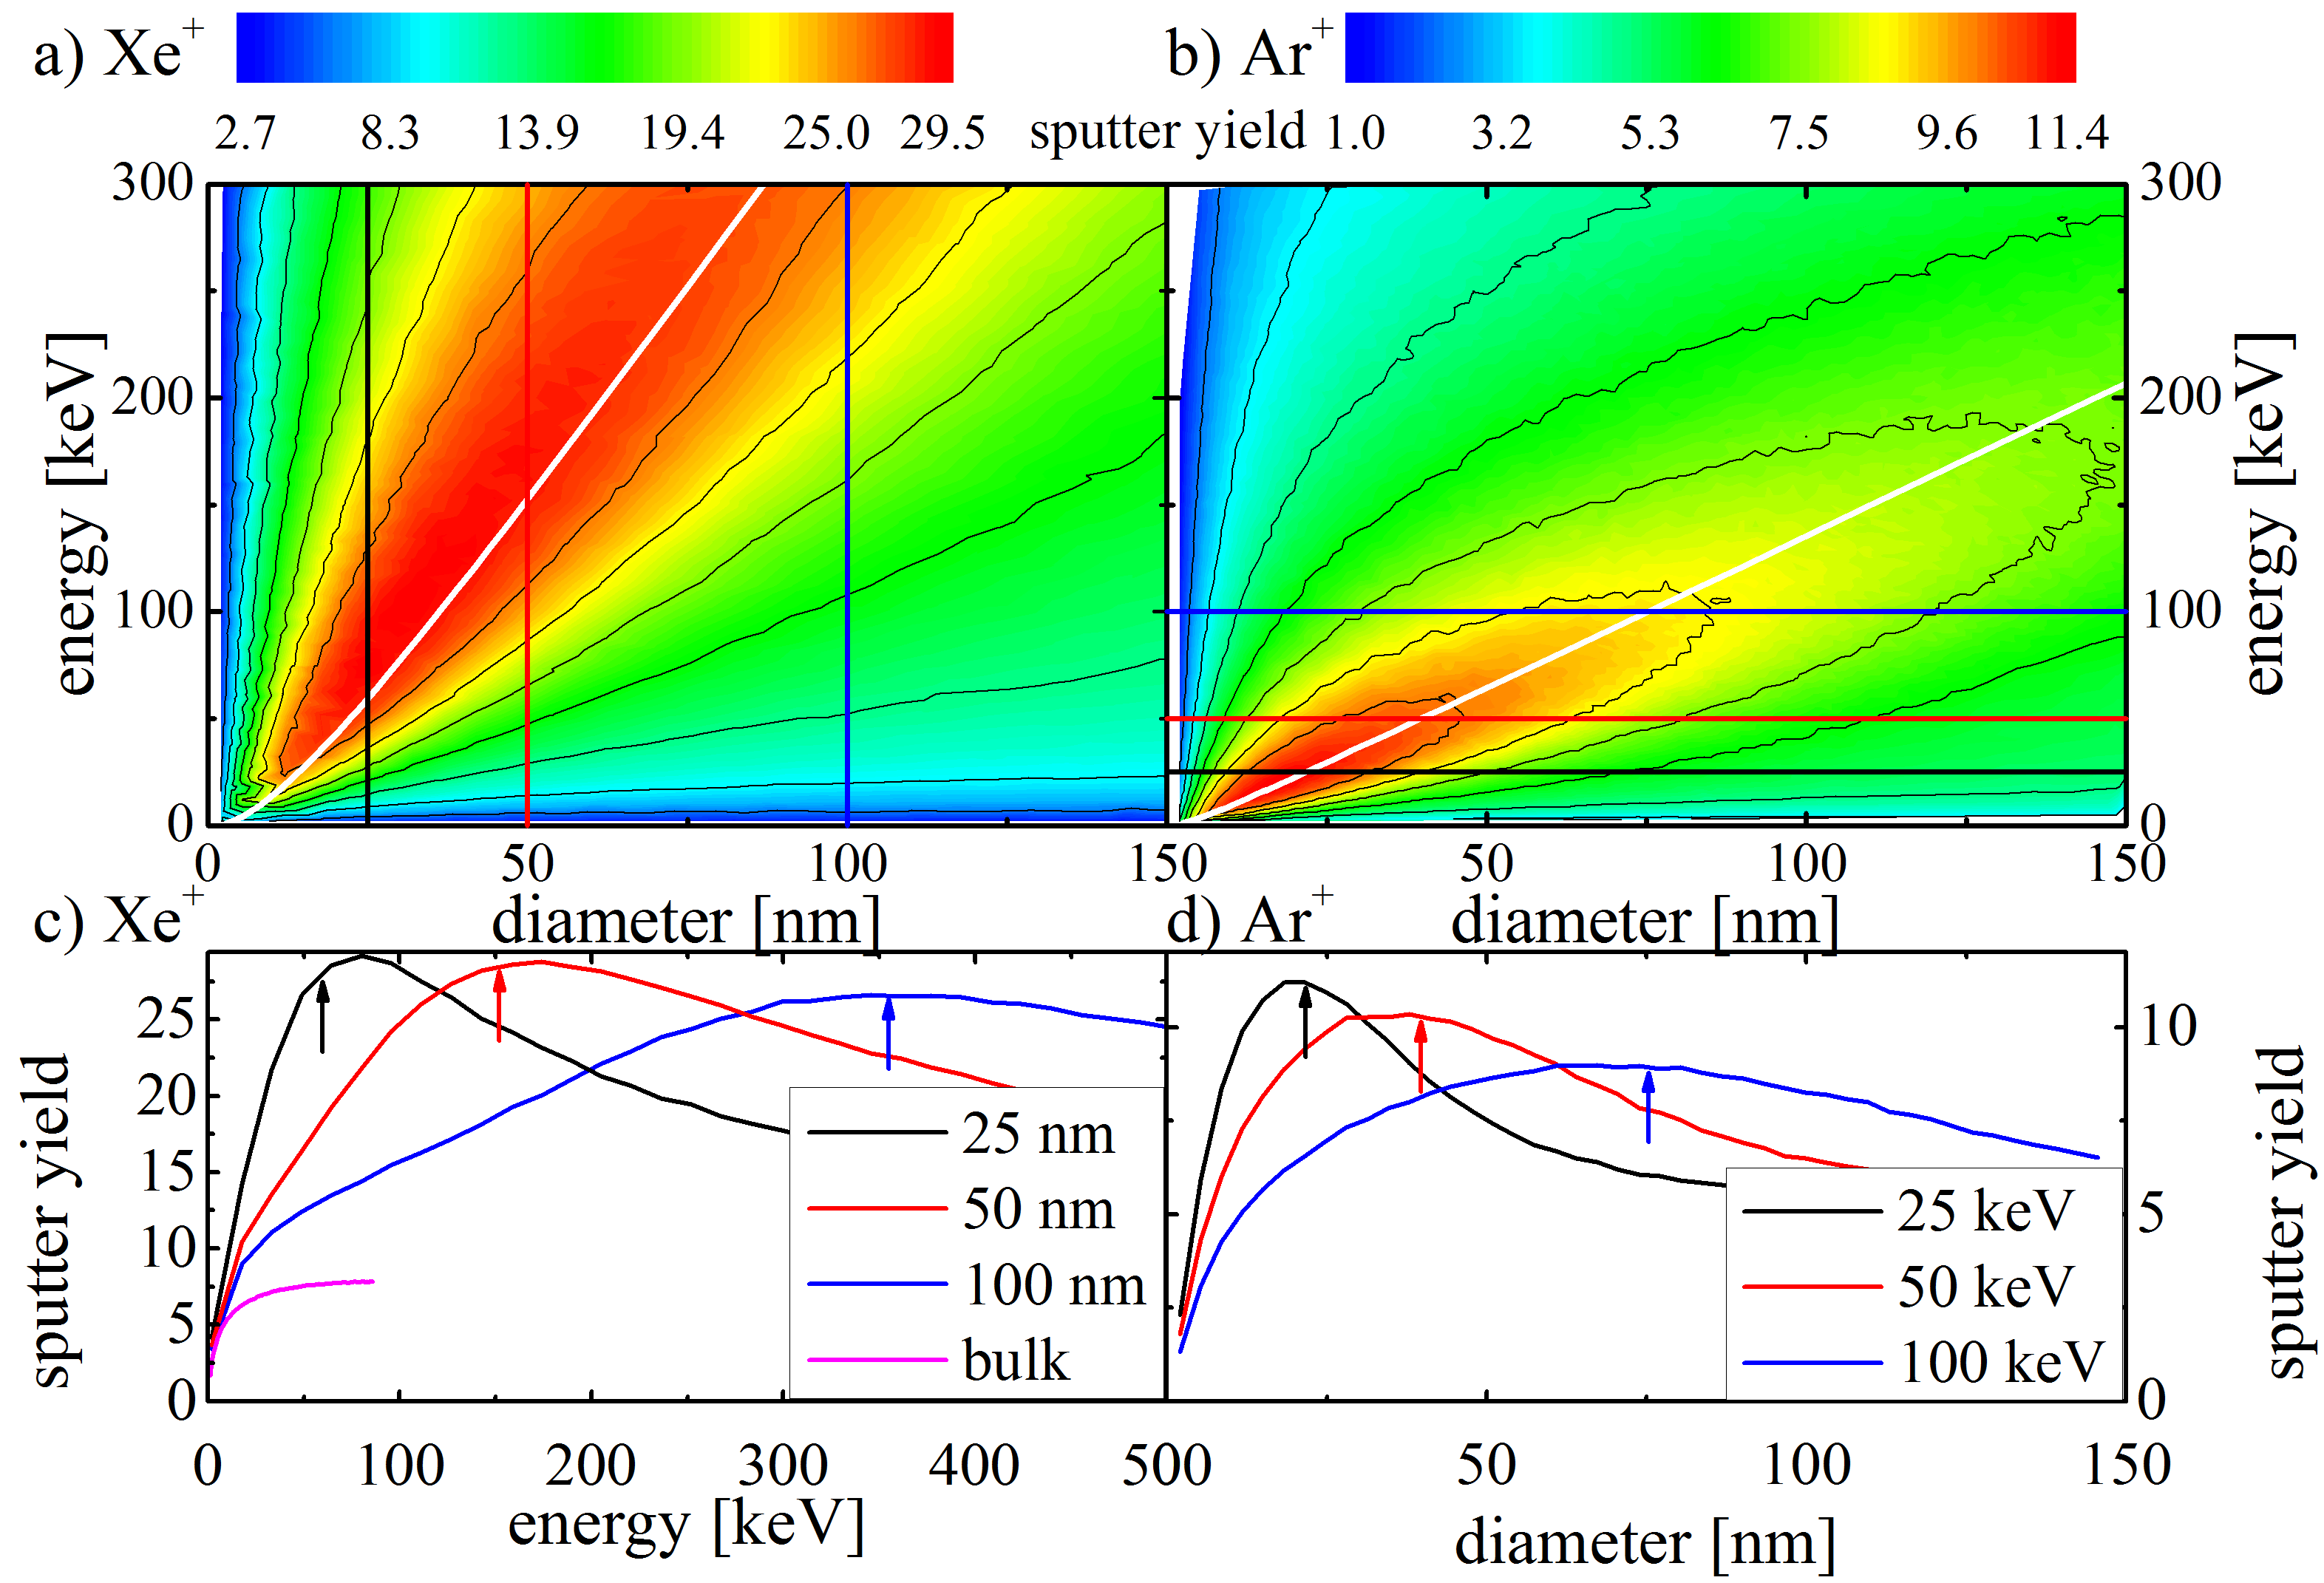
\includegraphics[width=.95\textwidth]{images/sputtering_diameter_energy.png}
	\caption{a) } 
	\label{sputtering_de}
\end{figure} 

In \ref{sputtering_de}c, the sputter yield versus energy is extracted from the $Xe^+$ simulation for set of fixed diameters. The red, blue and black curves correspond to the simulation of $25, 50$ and $100\,nm$ diameter wires, respectively. The corresponding vertical lines in figure \ref{sputtering_de}a show the position of the extracted data in the color plot. The maximum clearly shifts to larger ion energies for larger diameters. It is near the point, where the colored arrows indicate the energy for which the ion range, simulated by SRIM, is equal to the respective diameter. The magenta curve shows the energy dependent sputter yield for a flat $Si$ surface irradiated with $Xe^+$ ions at $45^\circ$, also simulated with \emph{iradina}. The broad maximum sputter yield for this bulk simulation is found at $\approx 100 \,keV$, correspondingly the global maximum sputter yield in nanowires is also found at $\approx 100 \,keV$ for $30\,nm$ diameter wires. Finally, in \ref{sputtering_de}d the sputter yield from $Ar^+$ irradiated $Si$ nanowires is plotted as a function of the diameter for a set of fixed energies. Here, the red, blue and black curves correspond to $25, 50$ and $100\,keV$ ions and the arrows indicate the ion range at the respective energy. Again the maximum sputtering is found at a diameter corresponding to the ion range in bulk.

To relate this to the Sigmund sputtering model with its Gaussian ellipsoid approximation of the damage profile, a Gaussian peak is fitted to the recoil profile simulated with SRIM for both ions in $Si$ \cite{bobes_ion_2012}. The so found mean damage depth is constantly around $0.7$ times the ion range for the whole energy range investigated here. A naive first approximation with the Sigmund sputtering model would predict that the sputtering is maximal where ions energy is such, that the mean depth of the damage and the radius of the irradiated nanowire coincide. However, this is only true for central impacts, while the simulated situation is an average over all ion-nanowire impact parameters. For non-central impacts there is less of the nanowire `in front' of the ion's path. Therefore, the maximum of the sputter yield is also at lower energies than it would be for solely central impacts. It is thus a coincidental consequence of the irradiation geometry that ion range is an even better predictor for the diameter of maximum sputtering than the center of the Gaussian fit to the damage distribution. To test the limits of the Sigmund model, a more thorough investigation of the Sigmund model's predictions for various irradiation scenarios may be interesting, however, since the MC simulations reproduce the reality more realistically anyhow, it will not be undertaken here.



\section{Redeposition}
\label{sec:redeposition}

While irradiating a nanowire which is standing perpendicular on a substrate as shown in \ref{} material will also be sputtered from the substrate. Some of the sputtered material from the substrate will be redeposited on the nanowire, so that the observable sputter yield will be lower than the actual sputtering. Consider the situation shown in figure \ref{redeposit}. An ion hits the substrate at point A. A possible path of a sputtered atom is indicated by the red line to a point on the nanowire, redepositing the substrate atom on the nanowire. 

\begin{SCfigure}
	\centering
		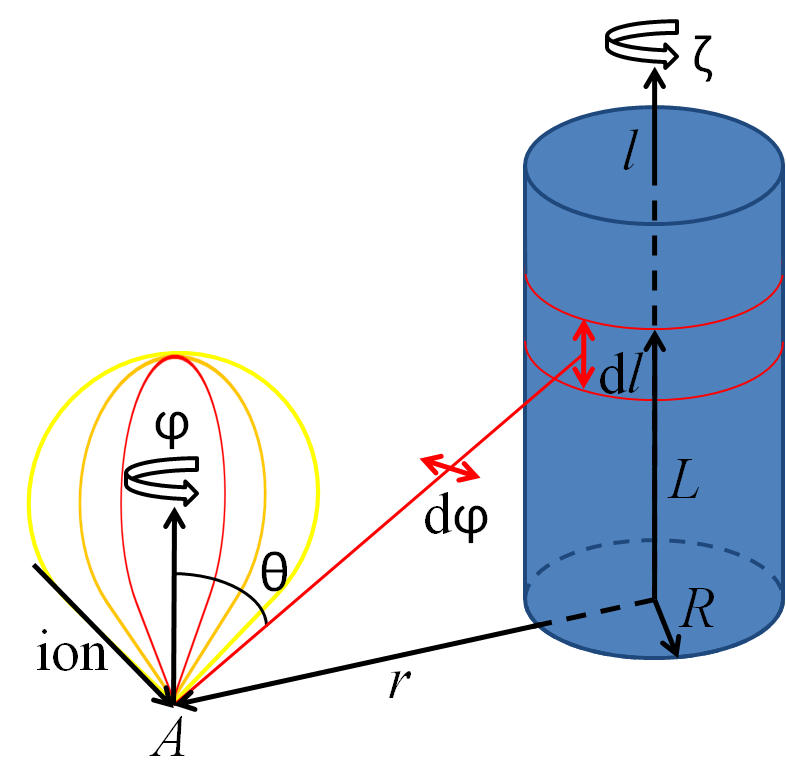
\includegraphics[width=.4\textwidth]{images/redeposit.jpg}
	\caption{Illustration of the redeposition of sputtered material from the substrate point A onto the nanowire with radius R at a height L. Since the wire is rotated around its axis $\zeta$ and the whole substrate is irradiated, a rotationally symmetric angle distribution for the sputtered atoms can be chosen.} 
	\label{redeposit}
\end{SCfigure}

The following calculation will estimate how many atoms are deposited on the nanowire, by first calculating the probability of a sputtered atom to hit it $P$:

\begin{equation}
\label{prob1}
P = \int_0^{2\pi} \! \,\int_0^{\pi/2} \!\! H(\theta,\varphi,r,R,L) \, \tilde{SY}(\theta,\varphi) \,cos(\theta)\,\mathrm{d}\theta \, \mathrm{d}\varphi.
\end{equation}

Where $H(\theta,\varphi,r,R,L)$ is the probability distribution of hitting the nanowire. It is $1/(4\pi)$ if the trajectory along $\theta$ and $\varphi$ from $r$ hits the nanowire with length $L$ and radius $R$, and zero otherwise. For irradiation at an angle, the angle distribution of the sputter yield $\tilde{SY}(\theta,\varphi)$ is expected to have a preferential direction along the ion beam \cite{verdeil_angular_2008}. However, the effective distribution becomes rotationally symmetric (independent of the angle $\varphi$) if one neglects the shadowing of the ion beam on the substrate. Then all points around the wire are hit and the wire is rotated around its axis (angle $\zeta$). This means that a rotationally symmetric angle distribution $\tilde{SY}(\theta)$ of the sputtered atoms from the substrate can be used, as indicated by the yellow, orange and red bulbs in figure \ref{redeposit}. A $cos^\kappa(\theta)$ distribution is chosen, as it forms flattened angle distributions for $\kappa < 1$, which can emulate the rotation of a slanted angle distribution: 

\begin{equation}
\tilde{SY}(\theta) = \frac{SY \cdot cos^\kappa(\theta)}{\int_0^{2\pi} \! \mathrm{d}\tilde\varphi \,\int_0^{\pi/2} \! cos^\kappa(\tilde\theta) cos(\tilde\theta)\,  \mathrm{d}\tilde\theta} \, = SY /c(\kappa) \cdot cos^\kappa(\theta) ,
\end{equation}

where the denominator $c(\kappa)$ normalizes the angle distribution function $cos^\kappa(\theta)$ and $SY$ is the total sputter yield from the surface. The parametrization of $H(\theta,\varphi,r,R,L)$ in $\varphi$ is straightforward, as the integration bounds for $\varphi$ are $[-\gamma, \gamma]$ with $\gamma = arcsin(R/r)$ the angle between $r$ and the tangent to the nanowire in figure \ref{anglesredepo}a. To solve the integration over $\theta$ it is useful to express the distance $q$ from the impact point to the base of the nanowire as a function of $\rho = R/r, r$ and $\varphi$:

\begin{equation}
q(\rho,r,\varphi) = r\cdot \sqrt{1 + \rho^2 - 2sin^2(\varphi) - \sqrt{cos^2(\varphi)(cos(2\varphi) - 1 + 2\rho^2)}}.
\end{equation}

\begin{figure}
	\centering
		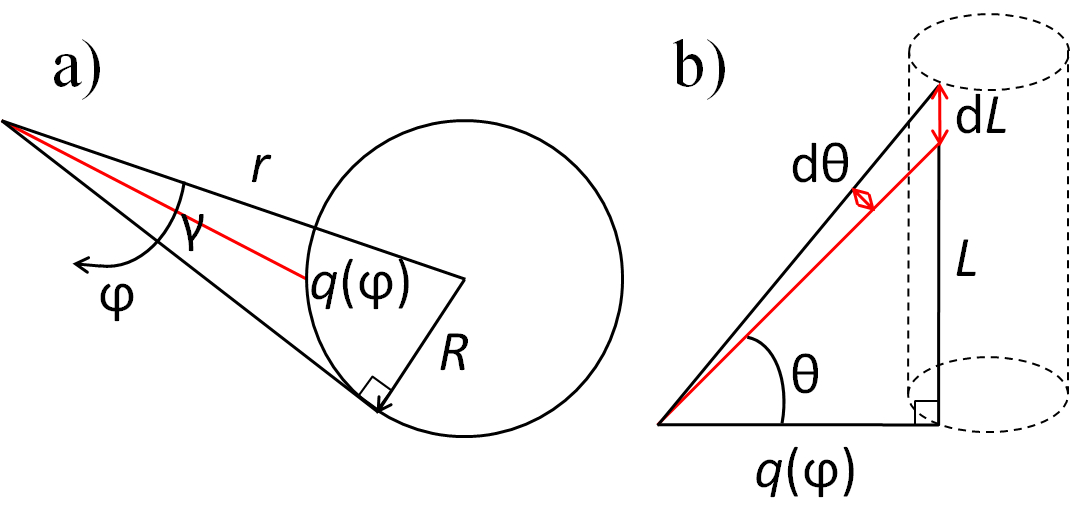
\includegraphics[width=.6\textwidth]{images/anglesredeposition.jpg}
	\caption{a) On the substrate surface $R$ is the radius of the nanowire, $r$ the distance from the point of impact A to the center of the wire, $q(\phi)$ the distance to the wires surface at the base of the wire. The angle between $r$ and the tangent to the nanowire circumference is $\gamma$. b) Side on view with $\theta$ the angle to the substrate normal of the trajectory to hit the wire at $L$.} 
	\label{anglesredepo}
\end{figure} 

Then the integration over $\theta$ can be substituted by an integration over the length of the nanowire $l$. The substitution can be found looking at figure \ref{anglesredepo}b:

\begin{align*}
\mathrm{d}\theta &= \frac{sin(\theta)}{\sqrt{L^2 + q^2}}\,\mathrm{d}L,\\
\theta &= arctan(q/L).
\end{align*}

Inserting into equation \ref{prob1} and simplifying yields:

\begin{equation}
\label{prob2}
P = \frac{2\,SY}{c} \int_0^{\gamma} \! \int_{L_1}^{L_2} \!  \frac{l^{\kappa+1}\,q}{(l^2 + q^2)^{(\kappa + 3)/2}} \,\mathrm{d}l \, \mathrm{d}\varphi.
\end{equation}

With $l^*=L_1-L_2$ the area hit on the nanowire is now $\pi \, R \, l^*$, positioned at the height $L= (L_1+L_2)/2$ as indicated between the two red lines in figure \ref{redeposit}. Integrating the probability $P$ to hit the nanowire at each substrate position over the whole substrate area and normalizing it to the area of the nanowire which is hit yields the number of atoms $N$ hitting the nanowire per fluence $\Phi$:

\begin{equation}
\label{prob3}
N/\Phi = \frac{2\,SY}{c \pi Rl^*} \int_0^{2\pi}\! \mathrm{d}\zeta \int_R^{\infty} \!
\int_0^{\gamma} \! \int_{L_1}^{L_2} \! r \frac{l^{\kappa+1}\,q}{(l^2 + q^2)^{(\kappa + 3)/2}}\,\,\mathrm{d}l \, \mathrm{d}\varphi\,\mathrm{d}r.
\end{equation}

The integration can be solved numerically using the numerical integration tools CQUAD and QAGI \cite{gough_gnu_2009}. Perhaps counter-intuitively, the result is independent of the nanowire radius $R$ and the height at $L$ at which the deposition is calculated. The redeposition amounts to $10\,\% \cdot \Phi\cdot SY$ for the very broad distribution when $\kappa = 0.25$. As already shown in figure \ref{sputtering_de}c, the sputter yield (SY) is significantly lower on the plane substrate than on the nanowire to begin with. Therefore, the redeposition can be safely neglected for the evaluation of sputtering. As the atoms sputtered from the substrate have a very low energy, they will be deposited on the surface of the nanowire. This makes them prone to re-sputtering, which reduces the finally incorporated number of substrate atoms even further. Nevertheless, care is advised in the choice of the substrate material, as the incorporation of substrate atoms in the nanowire may have detrimental doping effects.



% However, this can be made plausible by looking at figure \ref{anglesredepo}. There is no characteristic radius $R_c$ which would change any of the geometric relations in \ref{anglesredepo}a. Since the integration is over all the $r > R$, necessarily always starts at $P(R) =1/2$ and goes to $P(r\rightarrow \infty) =0$, its result is independent of $R$. For $L$ it can be argued in figures \ref{anglesredepo}b or \ref{redeposit} that for a fixed $\theta$, $\mathrm{d}L \propto 1/r$ scales as the inverse of the area $\mathrm{d}A \propto r$ of the annulus radiating towards the nanowire under that angle. Therefore the redeposition is constant along the whole nanowire length. 




\section{$Si$ nanowire sputtering by $Ar^+$ irradiation}
\label{sec:sisputtering}

The experimental verification of the diameter dependent maximum in sputtering was investigated on etched $Si$-nanowire arrays. Figure \ref{sputtering_exp}a shows the principle irradiation setup illustrated by a SEM image of a single nanowire before and after the irradiation with $300\,keV\,Ar^+$. The etched nanowire samples and the RHT allowed the simultaneous, rotated irradiation of upstanding nanowires with various diameters at $300\,^\circ C$. Figure \ref{sputtering_exp}b shows the extracted and aligned diameter versus height profile for the nanowire in figure \ref{sputtering_exp}a. More than $100$ such profiles were semi-automatically extracted for many different nanowire diameters. The sputter yield calculated from these extracted profiles is plotted versus the local diameter in \ref{sputtering_exp}c for $100$ and $300\,keV\,Ar^+$.

\begin{figure}[th]
	\centering
		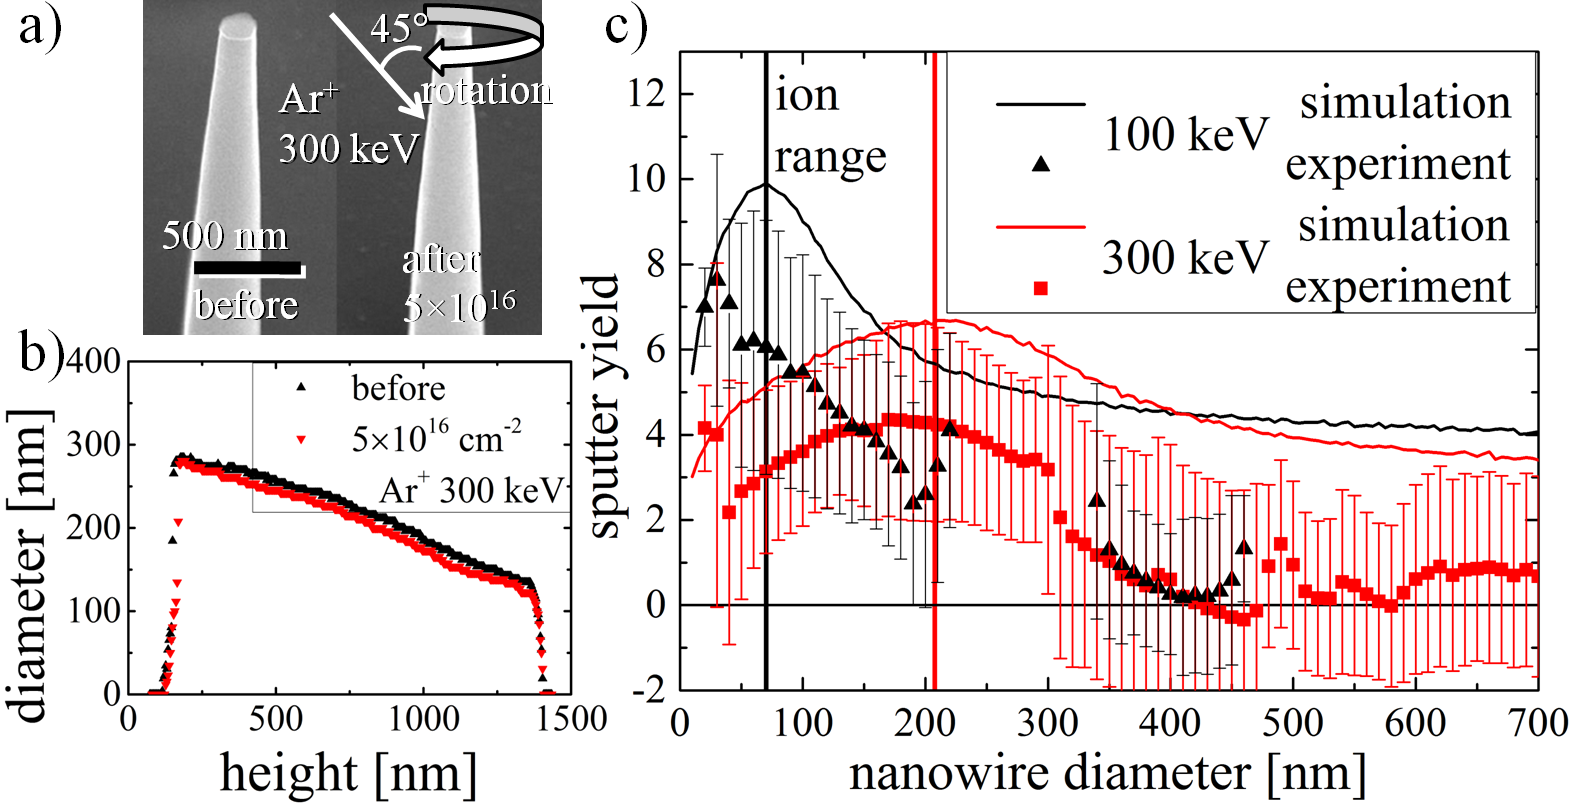
\includegraphics[width=.95\textwidth]{images/sputter_exp.png}
	\caption{a) Exemplary SEM images of a $Si$ nanowire before and after the rotated irradiation with $300\,keV\,Ar^+$ at $300^\circ C$. The extracted diameter vs. height profile for this nanowire is shown in b). From many such profiles the sputter yield vs. diameter was calculated and plotted in c) as black triangles and red squares for the irradiation with $100$ and $300\,keV\,Ar^+$, respectively. The `error bars' indicate the variance of the data points grouped together every $10\,nm$. The sputter yield calculated with \emph{iradina} simulations is shown for either case as a line-plot. The corresponding SRIM ion range at $45^\circ$ is marked by a vertical line.} 
	\label{sputtering_exp}
\end{figure} 

The experimental sputter yield reproduces the qualitative, simulated diameter dependence of the sputter yield well. The maximum sputtering is found for those nanowire diameters where the diameter corresponds to the ion range, just as discussed in chapter \ref{sec:simsputering} and the Sigmund sputtering model in chapter \ref{sec:ionsolid}. The interruptions and discontinuities for diameters $<50\,nm$, at $\approx 200\,nm$, $\approx 300\,nm$ and $\approx 500\,nm$ are located where the diameter range of an array of nanowires on the irradiated substrate ended. Here, there are fewer (none for 100\,keV and $\approx 200 - 300\,nm$) nanowires which could be evaluated.

The large variance indicated in figure \ref{sputtering_exp}c as `error-bars' can be attributed to the fact that the observed diameter changes of around $5\,nm$ are close to the resolution limit of the SEM, which is $2\,nm$. Therefore, the observation of a sensible sputter yield value is only possible with the large number, $>1000$, of diameters evaluated. Nevertheless, sputter yields around 0, as found in the experimental values at $400\,nm$ are not realistic. They have to be attributed to misalignment and remaining focal plane, brightness and contrast differences between the SEM images before and after irradiation which could not be corrected in the image analysis. Because of these systematic deviations, the variance is a more useful estimation at the accuracy of the experimentally determined sputter yield than the more usual standard deviation which would underestimate the experimental error considerably.



The quantitative discrepancy between the simulated sputter yield and the experimental values is not unexpected. To start with, the the quantitative value from the \emph{iradina} simulation was discussion in chapter \ref{sec:simion} to be questionable. Nevertheless, the main contribution to a systematic deviation in the experimentally evaluated sputter yields is the oxidation of the $Si$ nanowires in air between the subsequent irradiation and SEM investigation steps. The thickness of oxidized $Si$ on the surface of the nanowires is significant but dependent on uncontrolled factors such as humidity and temperature \cite{lukes_oxidation_1972,al-bayati_composition_1991}. As all the oxygen in the oxidized layer of the nanowires also has to be sputtered away, the experimental procedure will underestimate the sputter yield.

\begin{SCfigure}
	\centering
		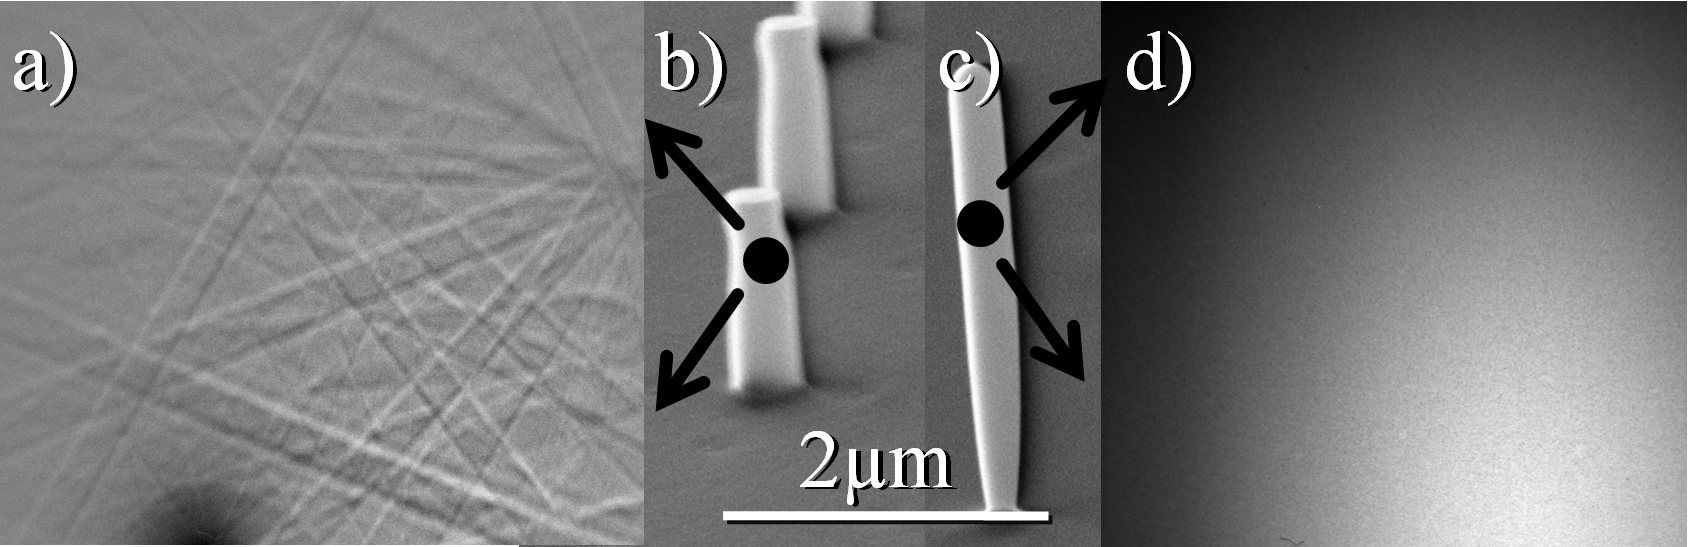
\includegraphics[width=.4\textwidth]{images/suppfig_EBSD.jpg}
	\caption{a) the EBSD pattern clearly shows that the nanowire shown in the SEM image b) has remained crystalline during the irradiation at $300^\circ C$. The nanowire shown in the SEM image c) was irradiated at room-temperature and amorphized, shown by the lack of a Kikuchi pattern in d).} 
	\label{EBSD}
\end{SCfigure}

Any effect of incorporated defects or even amorphization on the density of the $Si$ in the nanowires can be confidently discarded, as nanowires remained crystalline during the irradiation even up to the high fluence of $5\cdot 10^{16}\,cm^2$. This was expected from other irradiation studies \cite{pelaz_ion-beam-induced_2004} and confirmed by EBSD \ref{EBSD}.

Finally, the fact that the experimentally observed sputter yield has its maximum at slightly lower diameters than the simulated values for both the $100\,keV$ and $300\,keV$ irradiations may indicate the occurrence of cluster and thermal sputtering. Both have been predicted with MD simulations \cite{nietiadi_sputtering_2014,urbassek_sputter_2015,anders_sputtering_2015}, albeit in nanostructures with much smaller dimensions. As the kinetic energy of the ion is, on average, distributed to less material in nanowires with smaller diameters, both cluster and thermal sputtering are enhanced for smaller nanowire diameters.

\section{Summary}

Sputtering was investigated with MC simulations and quantified in experiments. MC simulations were performed with \emph{iradina} for the irradiation of $Si$-nanowires with varying diameters at $45^\circ$ with $Xe^+$ and $Ar^+$ at varying energy. The sputter yield shows a local maximum in the diameter and energy dependent sputtering where the energy dependent ion range is about equal to the diameter of the nanowire. This can be understood as the point where the overlap of the nuclear energy deposition and the surface of the nanowire is largest. For a fixed ion energy, the ion will pass through nanowires with a small diameter, limiting the amount of energy deposited as well as the surface area. For increasing diameters, both the surface area and deposited energy increase, until the diameter is so large that the collision cascade no longer reaches the back side of the nanowire and forward sputtering is suppressed. For arbitrarily large diameters sputtering is still larger in cylinders than flat surfaces due to the larger impact angle of off-center impacts. Qualitatively this shows that the Sigmund sputter model provides a reasonable first approximation for the diameter and energy dependence of sputtering.
 
Experiments on the sputtering of $Ar^+$ irradiated, etched $Si$ nanowire arrays were presented. The irradiation was performed at $300^\circ$ on a rotated stage tilted by $45^\circ$ preventing the amorphization and bending of the irradiated $Si$ nanowires. From high-resolution SEM images performed before and after the irradiation the diameter dependent sputter yield could be extracted for the irradiation at $100$ and $300\,keV$. The quantitative reproduction of the simulated sputter yields is not possible due to both experimental and theoretical constraints, however these experiments reliably reproduce a maximum in the diameter dependent sputtering. A theoretical investigation into the redeposition of sputtered material from the substrate onto the nanowires, shows that the redeposition is negligible and neither dependent of the nanowire radius nor length. The fact that the experimentally observed diameter of maximum sputtering is lower than theoretically predicted may indicate, that thermal and cluster sputtering are occurring.

